%\documentclass[aps,twocolumn,secnumarabic,balancelastpage,amsmath,amssymb,nofootinbib, floatfix]{revtex4}
\documentclass[aps,twocolumn,secnumarabic,balancelastpage,amsmath,amssymb,nofootinbib,floatfix]{revtex4-1}
\newcommand{\abs}[1]{\lvert#1\rvert}

\usepackage{graphicx}      % tools for importing graphics
%\usepackage{lgrind}        % convert program code listings to a form 
                            % includable in a LaTeX document
%\usepackage{xcolor}        % produces boxes or entire pages with 
                            % colored backgrounds
%\usepackage{longtable}     % helps with long table options
%\usepackage{epsf}          % old package handles encapsulated postscript issues
\usepackage{bm}            % special bold-math package. usge: \bm{mathsymbol}
%\usepackage{asymptote}     % For typesetting of mathematical illustrations
%\usepackage{thumbpdf}
\usepackage{lipsum} 
\usepackage[colorlinks=true]{hyperref}  
\DeclareMathOperator\erfc{erfc}
\graphicspath{{../../plots/102317_Batch_Ni/}{../../plots/pictures/}}

\begin{document}
\title{HFNG Flux Measurement by Foil Activation}
\author{Jonathan T. Morrell}
\email{jmorrell@berkeley.edu}
%\homepage{http://www.jonathanmorrell.info/} %If you don't have one, just comment out this line.
\date{\today}
\affiliation{University of California, Berkeley - Nuclear Engineering}
\setlength{\parskip}{1em}

\begin{abstract}
In this experiment we use the foil activation technique to measure the fast neutron flux in the Berkeley High Flux Neutron Generator (HFNG).  The irradiation began at 12:23 on 02/26/2018 and ended at 22:10 on 03/09/2018  The peak flux measured was (1.96$\pm$0.26)$\cdot 10^7$ [$\frac{n}{cm^2s}$] using the following monitor channel(s): $^{58}$Ni(n,p)$^{58}$Co.
\end{abstract}

\maketitle


\section{Overview}

The High-Flux Neutron Generator (HFNG), pictured in Fig. \ref{fig:hfng} is a DD-fusion neutron source operated by the University of California, Berkeley Nuclear Engineering department, located in Etcheverry Hall.  The facility is host to a wide range of users, with applications such as neutron activation analysis, cross-section measurements and geochronology.

DD neutron generators have a number of advantages over research reactors as a sources of neutrons: they are safer, cheaper, easier to build and operate, and the neutron flux spectrum in a neutron generator is nearly mono-energetic, with a well characterized energy-angle correlation.  Their principal disadvantage is that the peak flux achievable in a neutron generator is several orders of magnitude lower than in a reactor.  As such, the neutron flux is a typical figure of merit for a neutron generator, with the goal of getting as high a flux as possible.

\begin{figure}[htb]
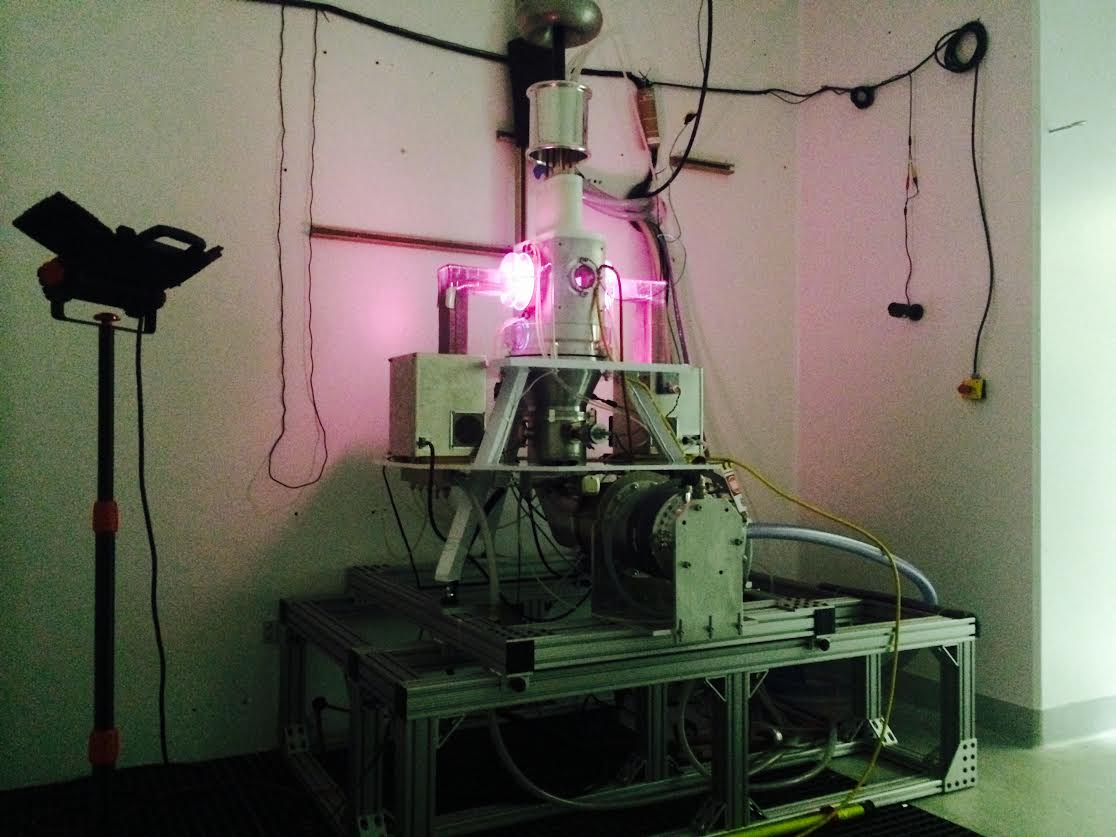
\includegraphics[width=7cm]{hfng.jpg}
\caption{Photo of the HFNG with both ion sources operating.
}
\label{fig:hfng}
\end{figure}

A variety of techniques exist for measuring neutron flux.  The technique used in this report is that of activation analysis of metal foils.  Disk-shaped samples are stamped out of thin metal foils, sealed inside of the HFNG target, and then irradiated for a chosen period of time.  The induced activity is measured by delayed $\gamma$-ray emission, counted using a high-purity Germanium (HPGe) detector.

The goal of this report is to give a detailed description of the determination of the neutron flux and energy spectrum in the HFNG, and present the results of this determination for a particular experiment.  This report presents the neutron energy and flux for each sample, followed by descriptions of the samples, detector calibrations, Monte-Carlo simulations of the flux spectrum, and a summary of the activation measured in each reaction channel of interest.

\subsection{Table of Fluxes}

For each sample irradiated in this experiment, the following table summarizes the uncertainty weighted average of the neutron flux measured in each observed reaction channel, as well as the flux-averaged neutron energy and the flux-weighted standard deviation of the neutron energy as determined by Monte Carlo methods.  Sample descriptions are provided in the next section. \\

\begin{ruledtabular}
\begin{tabular}{ccc}
Sample & Neutron Energy [MeV] & Flux [$\frac{n}{cm^2s}$] \\
\hline
1 & 2.755 $\pm$ 0.021 & (3.98$\pm$0.5)$\cdot 10^7$ \\
2 & 2.661 $\pm$ 0.035 & (4.77$\pm$0.6)$\cdot 10^6$ \\
3 & 2.607 $\pm$ 0.022 & (2.82$\pm$0.39)$\cdot 10^6$ \\
4 & 2.539 $\pm$ 0.006 & (3.02$\pm$0.46)$\cdot 10^5$ \\
5 & 2.247 $\pm$ 0.006 & (6.97$\pm$1.12)$\cdot 10^5$ \\

\end{tabular}
\end{ruledtabular}


\subsection{Sample Summary}

The following table lists the elemental composition and measured mass for each sample irradiated in this experiment, as well as the associated $\gamma$-spectrum file(s). \\

\begin{ruledtabular}
\begin{tabular}{cccc}
Sample & Element & Mass [g] & $\gamma$-Spectrum Filename \\
\hline
1 & Ni & 0.0847 & \texttt{\detokenize{Ni_NaCl_1.Spe}} \\
2 & Ni & 0.0908 & \texttt{\detokenize{Ni_NaCl_2.Spe}} \\
3 & Ni & 0.09 & \texttt{\detokenize{Ni_NaCl_3.Spe}} \\
4 & Ni & 0.3273 & \texttt{\detokenize{Ni_NaCl_4.Spe}} \\
5 & Ni & 0.3274 & \texttt{\detokenize{Ni_NaCl_5.Spe}} \\

\end{tabular}
\end{ruledtabular}

The following table lists the radius of each sample disk, as well as the coordinates of the sample inside the HFNG target relative to the origin of the (left side) beam spot.  $\Delta \theta$ indicates angle relative to the normal vector of the beam, which should only be non-zero if the sample-holder used was elbowed. \\

\begin{ruledtabular}
\begin{tabular}{cccccc}
Sample & $R$ [mm]& $\Delta$x [mm] & $\Delta$y [mm] & $\Delta$z [mm] & $\Delta \theta$ [$^{\circ}$] \\ 
\hline
1 & 4.0 & -9.75 & 9.75 & 8.5 & 0 \\
2 & 4.0 & 9.75 & 9.75 & 8.5 & 0 \\
3 & 4.0 & -9.75 & -9.75 & 8.5 & 0 \\

\end{tabular}
\end{ruledtabular}

\subsection{Methodology}

The general methodology of the thin-foil activation technique proceeds as follows.  First the samples are stamped out of metal foils into thin disks, having mass $m$ and number density

\begin{equation}
n=\frac{w\cdot m \cdot N_A}{M}
\label{eq:number_density}
\end{equation}
where $w$ is the isotopic abundance in the sample, $M$ is the molar mass and $N_A$ is Avagadro's number.  The sample is usually chosen to have a reaction channel (or multiple channels) with a high cross-section in the DD energy range, about 2-3 MeV, and a half-life comparable to the duration of the irradiation.

Following irradiation, the flux is determined by the ratio of the induced activity to the cross-section, number density and the fraction of saturation activity $F_S$.

\begin{equation}
\phi = \frac{A_0}{\sigma n F_S}
\label{eq:flux_calc}
\end{equation}

This represents an average flux, integrated over the area of the sample, the neutron energy spectrum, and over the total irradiation time of the experiment.

If the irradiation takes place in a single, continuous run of time $t_i$ then the saturation fraction will simply be $F_S = (1-e^{-\lambda t_i})$, where $\lambda$ is the decay constant of the reaction product.  If the irradiation is broken up into multiple cycles, the saturation fraction will be a recursive function of the cumulative irradiation history.

The induced activity is determined by delayed $\gamma$-ray counting using an HPGe detector.  If a $\gamma$ spectrum is counted for a measurement time $t_m$, beginning some amount of time $t_c$ after the neutron beam was shut off, then the end-of-beam activity measured in a photo-peak having $N_c$ counts will be

\begin{equation}
A_0 = \frac{\lambda N_c}{(1-e^{-\lambda t_m})e^{-\lambda t_c}I_{\gamma}\epsilon}
\label{eq:activity}
\end{equation}

where $I_{\gamma}$ is the $\gamma$ emission fraction per decay and $\epsilon$ is the detector efficiency at that particular photo-peak energy.

Because the neutron energy spectrum $\psi(E)$ over each sample isn't purely mono-energetic, the cross-section used in the flux calculation should be an averaged cross-section $\bar{\sigma}$ given by

\begin{equation}
\bar{\sigma} = \frac{\int_0^{\infty}\sigma\psi(E)dE}{\int_0^{\infty}\psi(E)dE}
\label{eq:avg_xs}
\end{equation}

The flux spectrum used can be determined by Monte Carlo methods, and is discussed later in this report.

\section{Irradiation History}

The following table lists the start and stop times for each cycle in this experiment, as well as the total number of hours during that interval. \\

\begin{ruledtabular}
\begin{tabular}{ccc}
Start & Stop & Total Time [h] \\ 
\hline
12:23 02/26/2018 & 14:14 02/26/2018 & 1.9 \\
14:28 02/26/2018 & 19:44 02/26/2018 & 5.3 \\
12:29 03/05/2018 & 21:12 03/05/2018 & 8.7 \\
09:41 03/06/2018 & 13:59 03/06/2018 & 4.3 \\
14:19 03/06/2018 & 22:31 03/06/2018 & 8.2 \\
08:27 03/07/2018 & 22:30 03/07/2018 & 14.1 \\
08:51 03/08/2018 & 22:41 03/08/2018 & 13.8 \\
09:35 03/09/2018 & 22:10 03/09/2018 & 12.6 \\
\end{tabular}
\end{ruledtabular}

This was used to calculate the saturation fraction, $F_S$ discussed previously.  The resulting calculation of $F_S$ as a function of the experiment time is plotted below for each reaction channel.

\begin{figure}[htb]
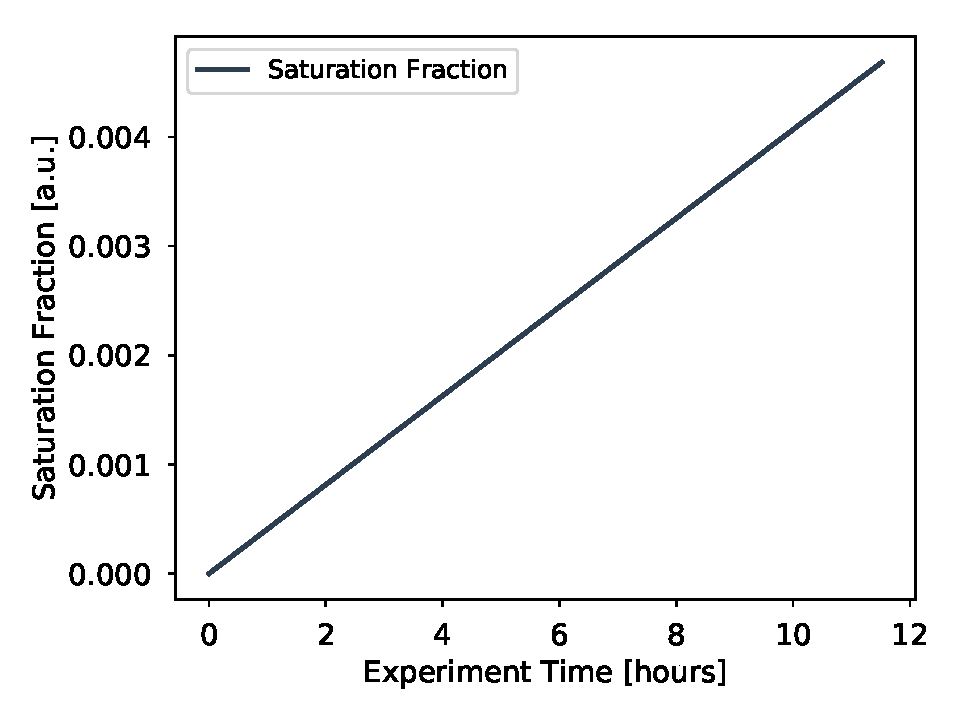
\includegraphics[width=9cm]{monitors/58CO_batemann}
\caption{Saturation fraction, $F_S$ for the $^{58}$Co isotope during the irradiation period.
}
\label{fig:58CO_batemann}
\end{figure}

The saturation fraction was calculated in an iterative manner according to the following procedure.  For a set of $N$ irradiation cycles with start times $S_n$ and stop times $P_n$, the saturation factor during a period of irradiation is given by

\begin{equation}
F_n(t_i) = 1 - (1-I_{n-1}e^{-\lambda(t_i-[P_{n-1}-S_0])})
\end{equation}

and during a period of decay (between irradiations) is given by

\begin{equation}
F_n(t_d) = I_{n-1}e^{-\lambda (t_d-[P_{n-1}-S_0])}
\end{equation}

where the constants $I_n$ are recursively determined by 

\begin{equation}
I_n = 1-(1-I_{n-1}e^{-\lambda (P_n-P_{n-1})})e^{-\lambda (P_n-S_n)}
\end{equation}

where $I_1=0$.  The saturation factor used to calculate the flux is simply $F_S=I_N$, i.e. the saturation factor corresponding to the last irradiation cycle.


\section{Calibration}
The energy and efficiency of the HPGe detector used in this measurement were calibrated using a standard calibration source of known activity (rel. error $<$1\%).  Additionally the peaks used in the calibration were used to characterize the resolution of the detector (and associated signal processing units).

A linear calibration of the $\gamma$-ray energy $E$ to the MCA channel number $N$, $E = m\cdot N+b$, was applied, and a plot of the residuals (Fig. \ref{fig:energy_calibration}) shows that this is the correct functional form of the energy calibration, i.e. that there is no quadratic component to the detector response.

\begin{figure}[htb]
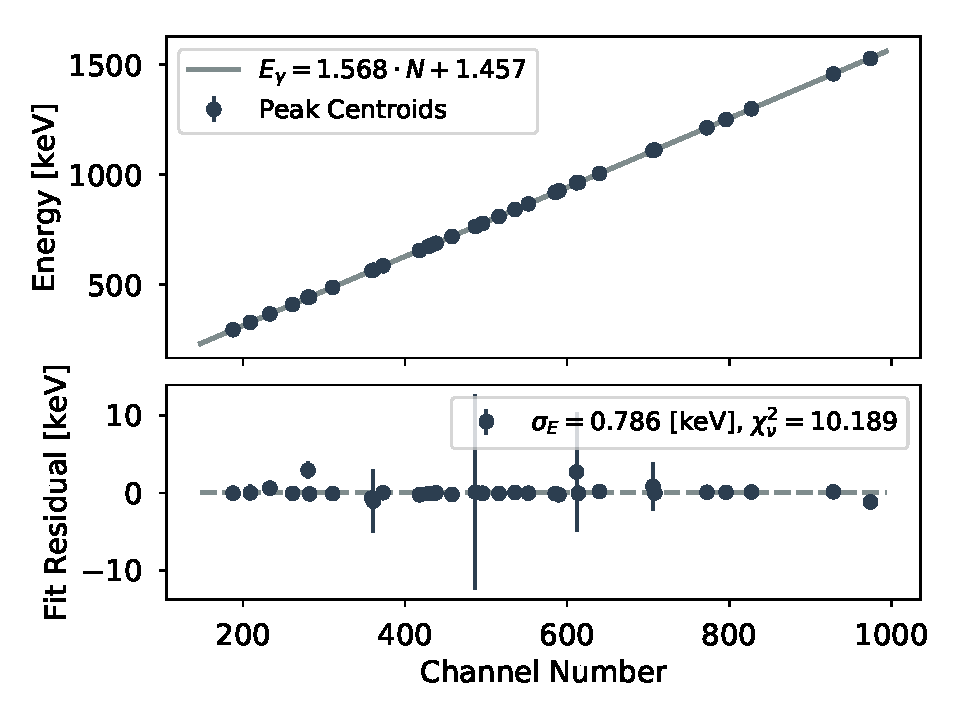
\includegraphics[width=9cm]{calibration/energy_calibration.pdf}
\caption{Linear energy calibration, and plot of the fit residuals.
}
\label{fig:energy_calibration}
\end{figure}

A modified 2$^{nd}$ order polynomial was applied for the detector efficiency calibration according to the equation

\begin{equation}
\epsilon (E) = exp[a\cdot ln(E)^2+b\cdot ln(E)+c]
\end{equation}

where $\epsilon$ is the efficiency and $a$, $b$, and $c$ are fitting constants.  The resulting fit for the detector efficiency used in this experiment is plotted in figure \ref{fig:efficiency_calibration}, showing reasonably good agreement.

\begin{figure}[htb]
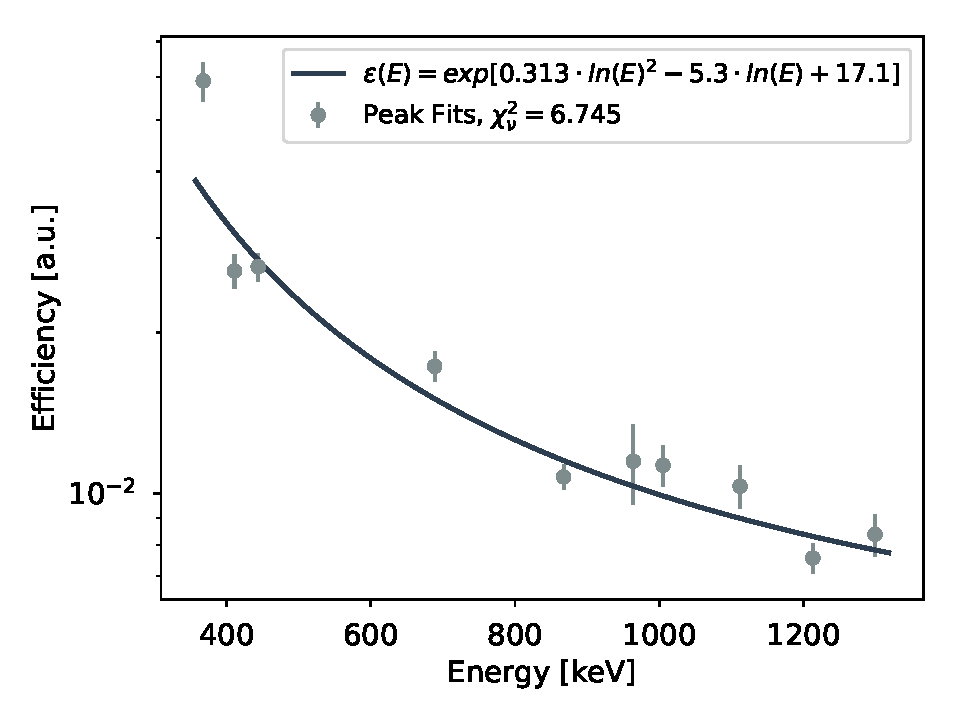
\includegraphics[width=9cm]{calibration/efficiency_calibration.pdf}
\caption{Detector efficiency calibration, relative to $\gamma$ emitting efficiency standard of known activity.
}
\label{fig:efficiency_calibration}
\end{figure}

The resolution for a HPGe detector should be proportional to the square root of the $\gamma$ energy, or in terms of the MCA channel number $N$ for a linear calibration

\begin{equation}
\sigma = \delta\sqrt{N}
\label{eq:resolution}
\end{equation}

where $\delta$ is a proportionality constant, usually a few percent.  The fit to equation \ref{eq:resolution} is plotted in figure \ref{fig:resolution_calibration}, below.

\begin{figure}[htb]
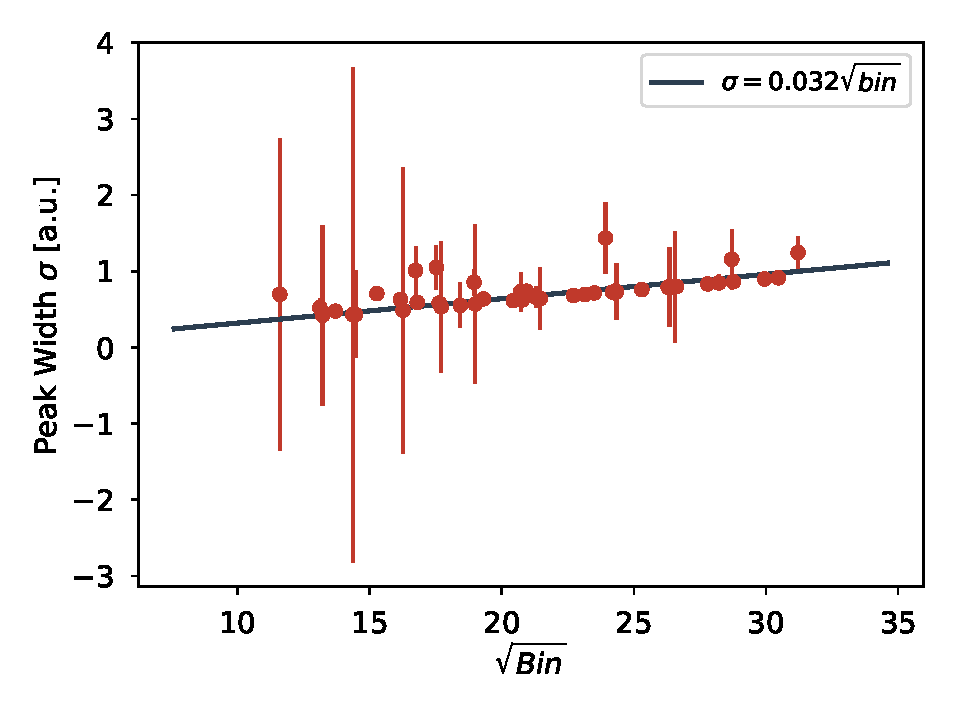
\includegraphics[width=9cm]{calibration/resolution_calibration.pdf}
\caption{Detector resolution calibration, and fit to equation \ref{eq:resolution}.
}
\label{fig:resolution_calibration}
\end{figure}


\section{Monitor Foil Characterization}

In order to choose a value for a tabulated reaction cross-section with which to calculate the average neutron flux on a foil, the neutron energy spectrum must be known either from measurement or calculation.  The approach taken in this experiment was to use a Monte Carlo model to calculate this flux spectrum.

In this model, scattering and absorption were treated as negligible as neutrons traverse less than 1 mfp through the HFNG target before reaching the foils.  The four physical effects considered in this model were the radial distribution of the neutron beam, the energy-angle correlation of the neutron source, the intensity-angle correlation, and the solid angle.

The flux spectrum for each sample was evaluated using the Monte Carlo method, a numerical technique for evaluating definite integrals.  The flux spectrum in a sample can be seen as an integral of a source distribution $S(\vec{r},E,\hat{\Omega})$ over space $d^3r$ and solid angle $d\hat{\Omega}$.  This can be rewritten as a Monte Carlo sum using the definition of the integral

\begin{align*}
\bar{\phi}(E) &= \int \int S(\vec{r},E,\hat{\Omega})d^3rd\hat{\Omega} \\
              &= \int \int \phi_0 \frac{n(\vec{r})\delta (\hat{\Omega}-\Omega_{sample})R(\theta(E))}{|\vec{r}-r|^2} d^3rd\hat{\Omega} \\
              &= \frac{1}{N} \sum_{n=1}^{N} \phi_0 \frac{R(\theta(E_n))\delta_{r\theta}}{(\Delta r_n)^2} = \phi_0 \sum_{n=1}^{N} \frac{R(\theta(E_n))\delta_{r\theta}}{(\Delta r_n)^2}
\end{align*}
where $n(\vec{r})$ is PDF for source (e.g. Gaussian) and $\delta_{r\theta}$ constrains neutron rays to source-sample paths.

The energy angle correlation used in this method is well-characterized, and is described using a four term polynomial

\begin{equation}
E_n(\theta) = A_0 + \sum_{n=1}^3 A_n cos^n(\theta)
\end{equation}

where the coefficients $A_n$ are given by the following table. \\

\begin{ruledtabular}
\begin{tabular}{ccc}
$A_n$ & 100 keV & 200 keV \\ 
\hline 
$A_0$ & 2.4674 & 2.47685 \\ 
$A_1$ & 0.30083 & 0.39111 \\ 
$A_2$ & 0.01368 & 0.04098 \\ 
$A_3$ & 0.0 & 0.02957 \\ 
\end{tabular}
\end{ruledtabular}

These coefficients can be interpolated based on the exact $D^+$ beam energy determined by the voltage on the cathode.  Figure \ref{fig:energy_angle} plots this correlation over all outgoing neutron angles, although most samples are at low angles.

\begin{figure}[htb]
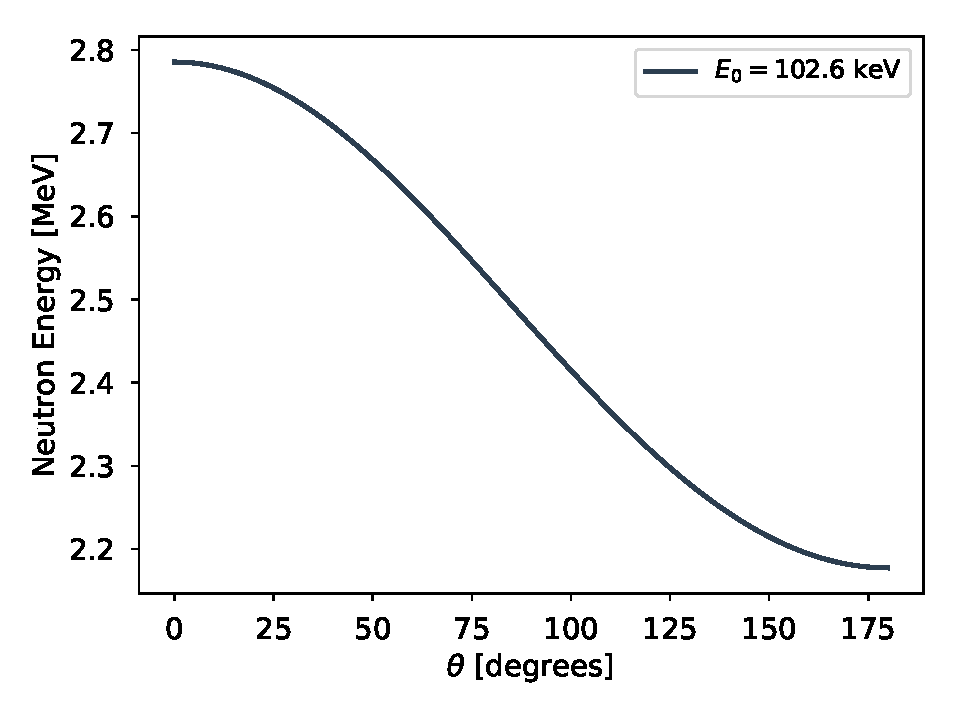
\includegraphics[width=9cm]{monitors/energy_angle.pdf}
\caption{DD fusion neutron emission energy angle correlation for the incident deuteron beam energy used in this experiment.
}
\label{fig:energy_angle}
\end{figure}

A similar, 6 term polynomial can be used to describe the relative intensity, or yield, as a function of angle:

\begin{equation}
\frac{R(\theta)}{R(90^{\circ})}=1+\sum_{n=1}^5 A_n cos^n(\theta)
\label{eq:intensity}
\end{equation}

where $\frac{R(\theta)}{R(90^{\circ})}$ is the ratio of emission at angle $\theta$ to $90^{\circ}$.  The polynomial coefficients $A_n$ are listed in the following table. \\

\begin{ruledtabular}
\begin{tabular}{ccc}
$A_n$ & 100 keV & 200 keV \\ 
\hline 
$A_1$ & 0.01741 & -0.03149 \\ 
$A_2$ & 0.88746 & 1.11225 \\ 
$A_3$ & 0.22497 & 0.38659 \\
$A_4$ & 0.08183 & 0.26676 \\
$A_5$ & 0.37225 & 0.11518 \\ 
\end{tabular}
\end{ruledtabular}

A plot of equation \ref{eq:intensity} using the coefficients for the incident beam energy set in this experiment is shown in Figure \ref{fig:intensity_angle}.

\begin{figure}[htb]
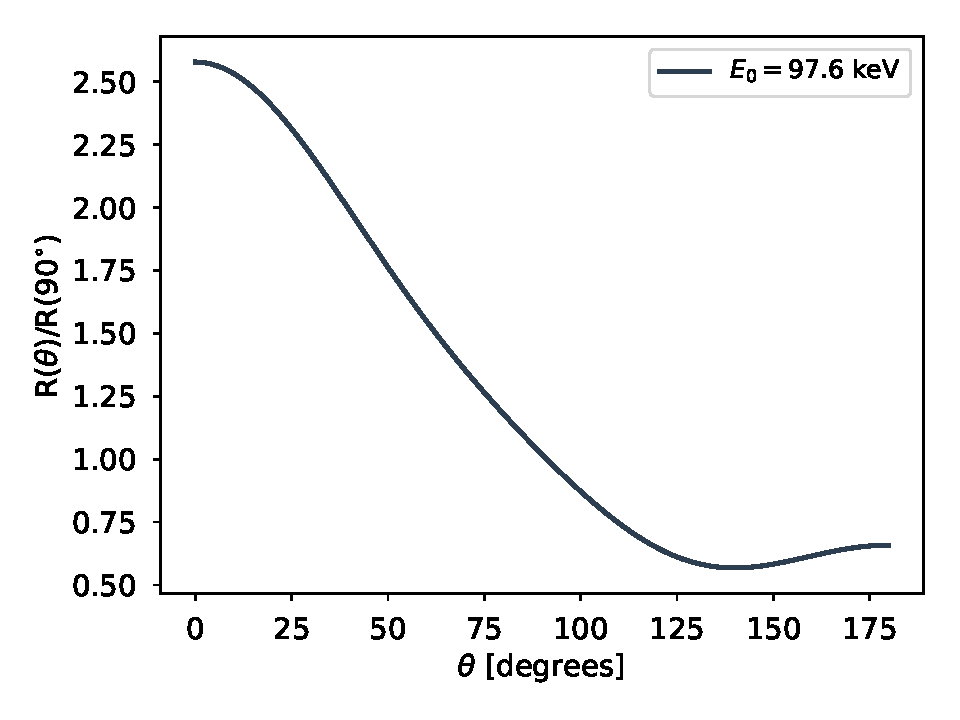
\includegraphics[width=9cm]{monitors/intensity_angle.pdf}
\caption{DD fusion neutron emission intensity angle correlation for the incident deuteron beam energy used in this experiment.
}
\label{fig:intensity_angle}
\end{figure}

Coordinates for the neutron rays were randomly generated from a Gaussian distribution with a radius determined by measurements of the beam-spot size on the target.  The sample coordinates were generated from a uniform distribution, but the correct spatial profile was achieved by weighting each tally according to the intensity-angle correlation and the distance squared.

Using these randomly generated coordinates, the emission angle can be calculated according to the definition of a dot-product of two vectors

\begin{equation}
\theta = arccos(\frac{\vec{r_1}\cdot\vec{r_2}}{|\vec{r_1}||\vec{r_2}|})
\end{equation}

where $\vec{r_1}$ is the normal vector to the neutron beam, and $\vec{r_2}$ is the vector connecting the source and sample coordinates.  An example in 2D is shown in Figure \ref{fig:MC_schematic}, where $\vec{r_1}=\left< 0, \Delta z \right>$ and $\vec{r_2}=\left< \Delta x, \Delta z \right>$.

\begin{figure}[htb]
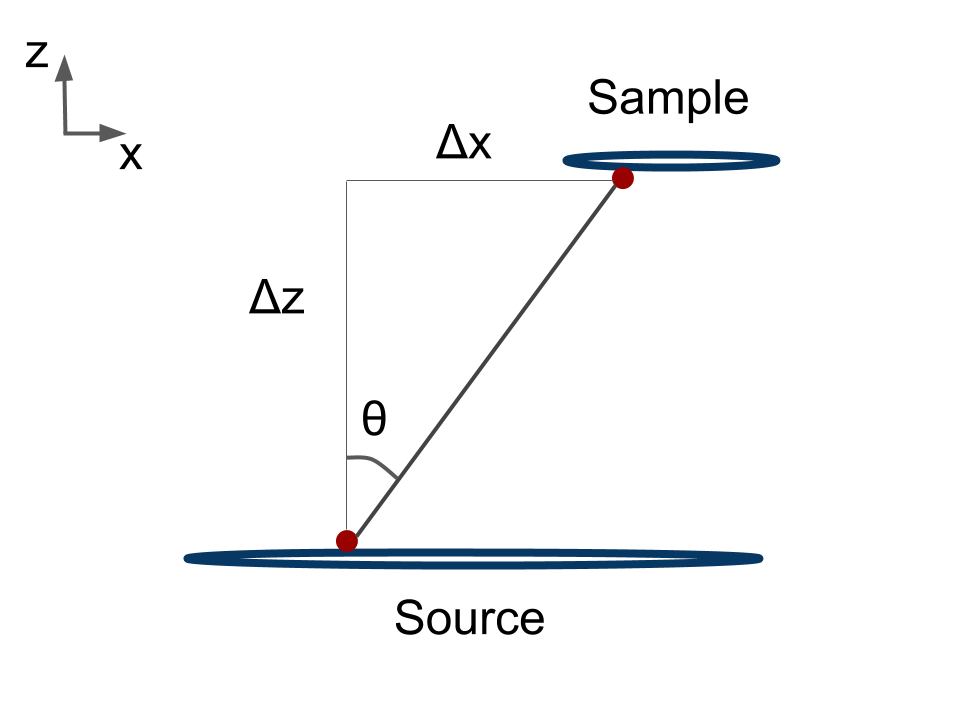
\includegraphics[width=9cm]{MC201_Graphic.png}
\caption{Schematic showing a 2D example of the randomly selected source and sample points that define the neutron ray.  The energy is determined by the angle, and the flux tally is weighted by the angular-intensity correlation and the square of the path length of the neutron ray.
}
\label{fig:MC_schematic}
\end{figure}

This method was applied for each sample using the geometry as described in the sample summary section, using 100,000 weighted flux tallies.  Plots of the resulting calculated flux spectra can be seen below, along with the mean energy and $\pm 1\sigma_E$ of the distribution.

\begin{figure}[htb]
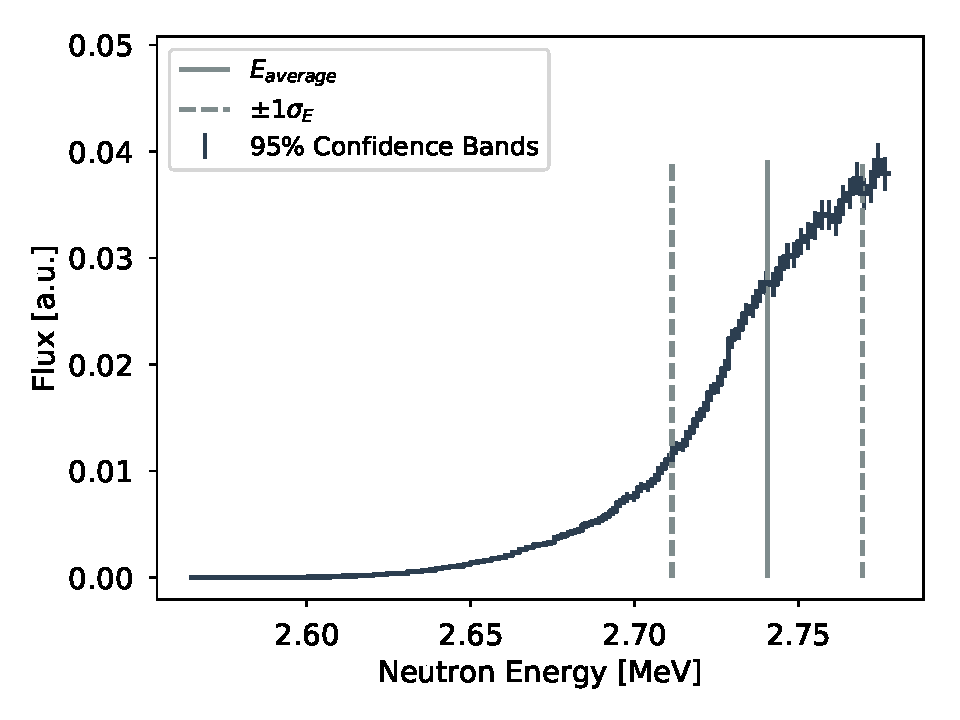
\includegraphics[width=9cm]{monitors/008False.pdf}
\caption{Energy spectrum, mean and $\pm 1\sigma_E$ for sample 1 calculated by Monte Carlo method.}
\label{fig:Spectrum1}
\end{figure}



This spectrum was then used to calculate an average cross-section for each reaction channel according to equation \ref{eq:avg_xs}.  The tabulated cross-sections used in this calculation were interpolated from the most recent EXFOR database.  Plots of these data, as well as the interpolated values and $\pm 1\sigma_{interp}$ can be seen in the figures below.

\begin{figure}[htb]
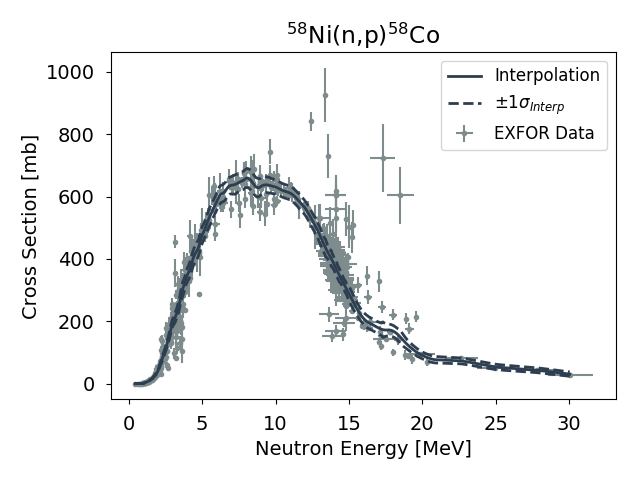
\includegraphics[width=9cm]{cross_sections/58NI_n_p_58CO}
\caption{$^{58}$Ni(n,p)$^{58}$Co cross section.  Data points are from EXFOR, solid/dashed lines are interpolated and $\pm 1\sigma$ values.
}
\label{fig:58NI_n_p_58CO}
\end{figure}

The resulting flux-averaged cross-section values for each sample and reaction channel are listed in the following table. \\

\begin{ruledtabular}
\begin{tabular}{cccc}
Sample & Reaction & Energy [MeV] & Cross-Section [mb] \\
\hline
1 & $^{58}$Ni(n,p)$^{58}$Co & 2.741 $\pm$ 0.029 & 149.7 $\pm$ 10.8 \\
2 & $^{58}$Ni(n,p)$^{58}$Co & 2.667 $\pm$ 0.044 & 137.2 $\pm$ 9.7 \\
3 & $^{58}$Ni(n,p)$^{58}$Co & 2.615 $\pm$ 0.035 & 128.8 $\pm$ 9.5 \\
4 & $^{58}$Ni(n,p)$^{58}$Co & 2.539 $\pm$ 0.009 & 116.4 $\pm$ 9.7 \\
5 & $^{58}$Ni(n,p)$^{58}$Co & 2.423 $\pm$ 0.017 & 99.6 $\pm$ 7.6 \\

\end{tabular}
\end{ruledtabular}


\section{Decay Curves}

For a single photopeak having $N_c$ counts observed with efficiency $\epsilon$ from a radioactive nucleus with decay constant $\lambda$ and intensity $I_{\gamma}$, equation \ref{eq:activity} can be used to calculate the end-of-beam activity for a given isotope.  However, if multiple photopeaks are to be used in the calculation the activity at some cooling time $t_c$ after the end-of-beam, the activity in a photopeak can be calculated by

\begin{equation}
A(t_c) = \frac{\lambda N_c}{(1-e^{-\lambda t_m})I_{\gamma}\epsilon}
\end{equation}

where $t_m$ is the measurement time.  The end-of-beam activity $A_0$ can then be calculated by a Levenberg Marquardt fit to the equation

\begin{equation}
A(t_c) = A_0e^{-\lambda t_c}
\end{equation}

The photopeak activities and exponential fits for each reaction channel of interest are plotted in the figures below.

\begin{figure}[htb]
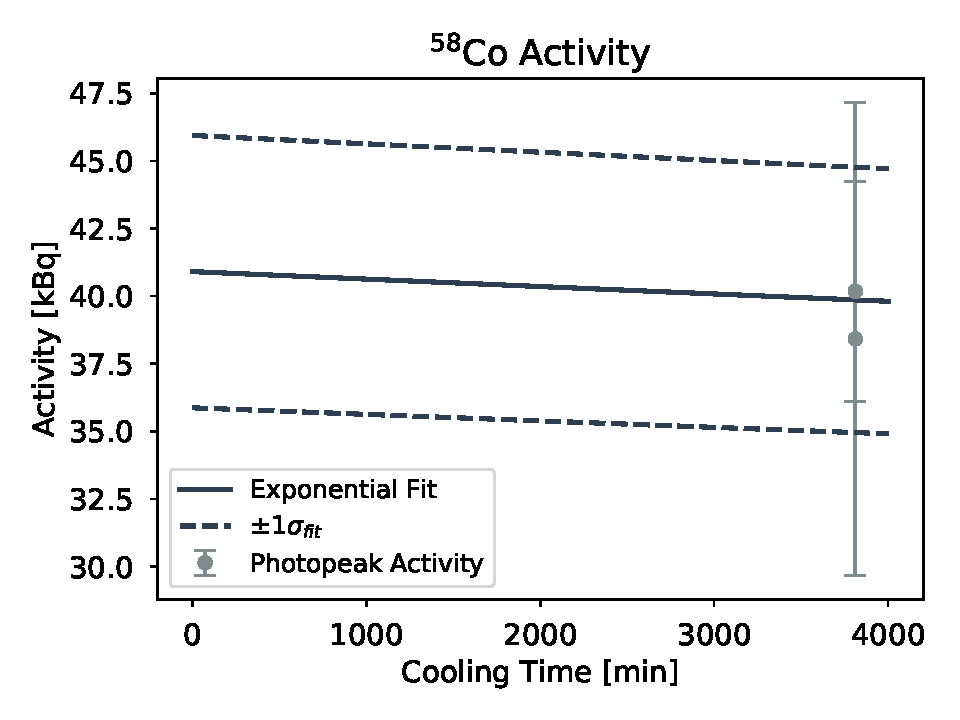
\includegraphics[width=9cm]{decay_curves/Ni_centered_58CO.pdf}
\caption{Exponential fit to the peak activities of $^{58}$Co measured in Sample 0.
}
\label{fig:Ni_centered_58CO}
\end{figure}



\section{Results}

Finally, the masses of each sample were determined by a high-precision digital scale, and using the values of $\sigma$, $A_0$ and $F_s$ discussed previously the flux values for each reaction channel in each sample were calculated using equation \ref{eq:flux_calc} and are listed in the following table. \\

\begin{ruledtabular}
\begin{tabular}{cccc}
Sample & Reaction & Energy [MeV] & Flux [$\frac{n}{cm^2s}$] \\
\hline
1 & $^{58}$Ni(n,p)$^{58}$Co & 2.741 $\pm$ 0.029 & (1.05$\pm$0.14)$\cdot 10^7$ \\
2 & $^{58}$Ni(n,p)$^{58}$Co & 2.667 $\pm$ 0.044 & (4.81$\pm$0.62)$\cdot 10^6$ \\
3 & $^{58}$Ni(n,p)$^{58}$Co & 2.615 $\pm$ 0.035 & (2.8$\pm$0.39)$\cdot 10^6$ \\
4 & $^{58}$Ni(n,p)$^{58}$Co & 2.539 $\pm$ 0.009 & (3.02$\pm$0.46)$\cdot 10^5$ \\
5 & $^{58}$Ni(n,p)$^{58}$Co & 2.423 $\pm$ 0.017 & (5.26$\pm$0.76)$\cdot 10^5$ \\

\end{tabular}
\end{ruledtabular}

The uncertainty weighted average of the flux determined by each reaction channel was calculated for each sample, giving the flux values tabulated at the beginning of this report.

\clearpage
\appendix
\onecolumngrid
\section{Peak Fits}
The detector energy and efficiency calibration, as well as the induced activity in each sample, was ultimately determined by peak fitting to the individual spectra.  Energy centroids and relative intensities were constrained with some uncertainty by the decay data given by the National Nuclear Data Center (NNDC).  Each peak was fit with a skewed Gaussian function on top of a linear background. Knoll recommends this as the functional form of a photopeak in an HPGe spectrum because localized charge trapping in the Ge crystal will lead to "tailing" on the low-energy side of the peak.  The complete functional form of the peak fit, $F(i)$, as a function of channel number $i$ is as follows.

The "background" under each photopeak, which could be due to actual background radiation or Compton scattering, was given a linear form:

\begin{equation}
F_{bg}(i) = m\cdot i + b
\label{eq:background}
\end{equation}

This is purely heuristic but is accurate in most cases because the background tends to be slowly varying over the energy range of one photopeak.  The resolution function for HPGe detectors is Gaussian, which means that the convolution of a photopeak (which can be assumed to be a delta function) with the resolution function simply gives a Gaussian peak shape:

\begin{equation}
F_{gauss}(i) = A\cdot \exp (-\frac{(i-\mu)^2}{2\sigma^2})
\label{eq:gaussian}
\end{equation}

where $A$ is the height of the peak, $\mu$ is the mean or centroid and $\sigma$ is the standard deviation, sometimes called the width of the peak.

The low energy tailing in an ideal detector is characterized by an exponential with argument $\frac{i-\mu}{\beta}$, where $\beta$ is a width parameter.  Convolution of this exponential with a Gaussian resolution function gives a skewed Gaussian:

\begin{equation}
F_{skew}(i) = B\cdot \exp (\frac{i-\mu}{\beta}) \erfc (\frac{i-\mu}{\sqrt{2}\sigma}+\frac{\sigma}{\sqrt{2}\beta})
\label{eq:skew}
\end{equation}

where $B$ is the height of the skewed Gaussian.  In general, $B$ is prortional to $A$, and $\beta$ is proportional to $\sigma$.  We will take advantage of this fact to better constrain our peak fits, as the number of parameters is already somewhat large.  Re-configuring the parameters $B$ and $\beta$ as $B = R\cdot A$, $\beta = \alpha \cdot \sigma$ means the parameters characterizing the skewed Gaussian will only have small variations between peaks and can be fit with much tighter bounds (i.e. faster).  For this experiment these skewed Gaussians were found to be approximately parameterized by $R \approx 0.2$ and $\alpha \approx 0.8$.

Finally, the complete equation for individual photopeaks is given by:

\begin{equation}
F_{peak}(i) = m\cdot i + b + A\cdot [\exp (-\frac{(i-\mu)^2}{2\sigma^2}) + R\cdot \exp (\frac{i-\mu}{\alpha \sigma}) \erfc (\frac{i-\mu}{\sqrt{2}\sigma}+\frac{1}{\sqrt{2}\alpha})]
\label{eq:peak}
\end{equation}

Below are plots of the $\gamma$-ray spectra for the samples and calibration sources, with photo-peak fits superimposed on the spectrum.

\begin{figure}[htb]
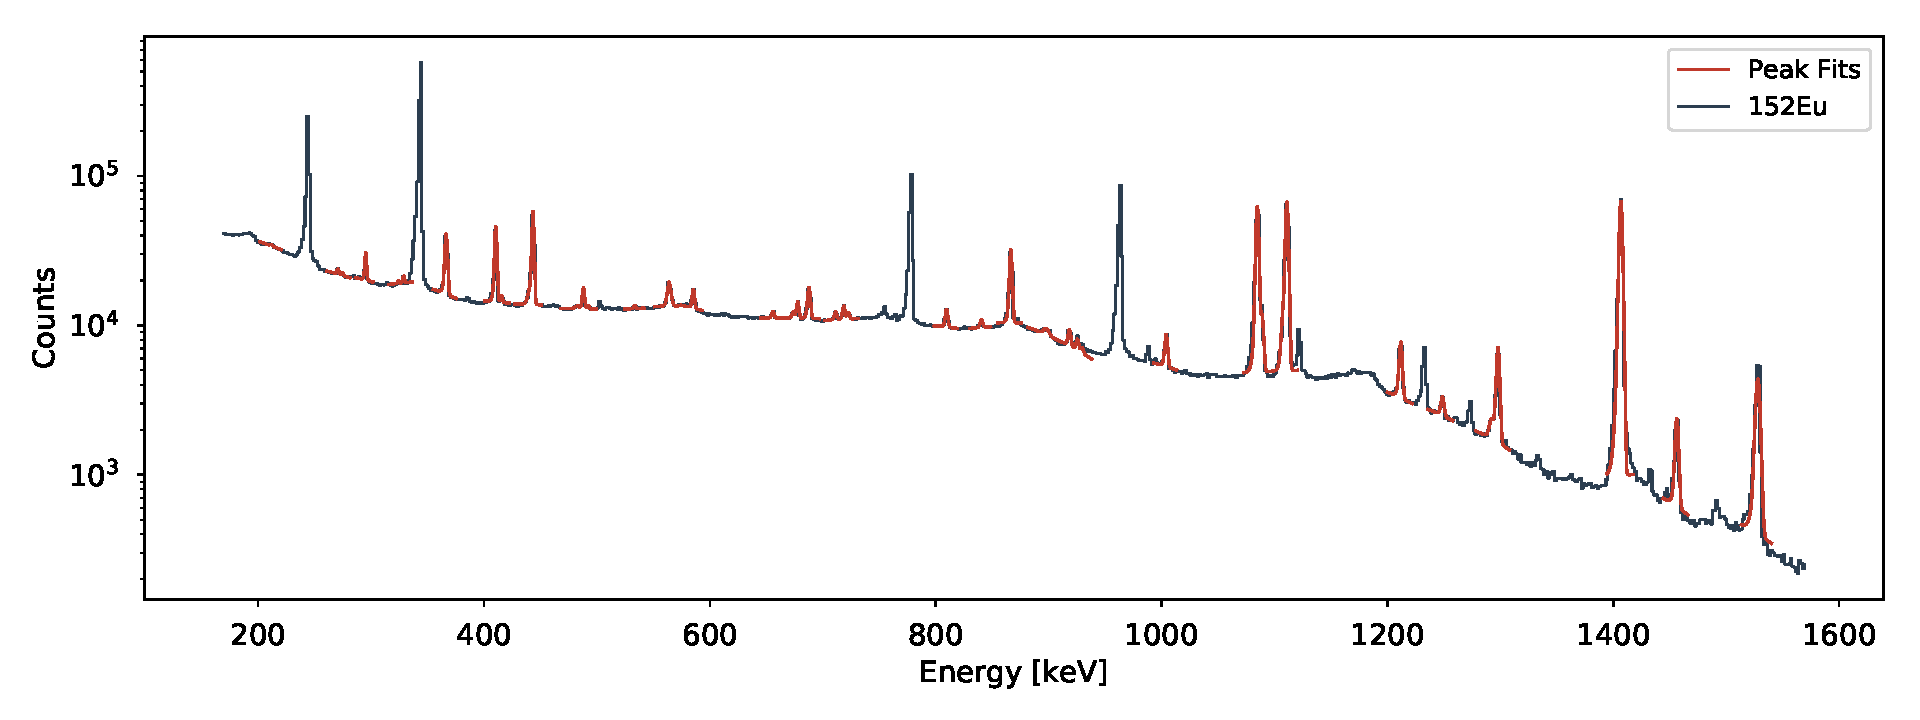
\includegraphics[width=\textwidth]{peak_fits/152Eu.pdf}
\caption{$\gamma$-ray energy spectrum and peak fits in \texttt{\detokenize{152Eu.Spe}}}
\label{fig:152Eu}
\end{figure}

\begin{figure}[htb]
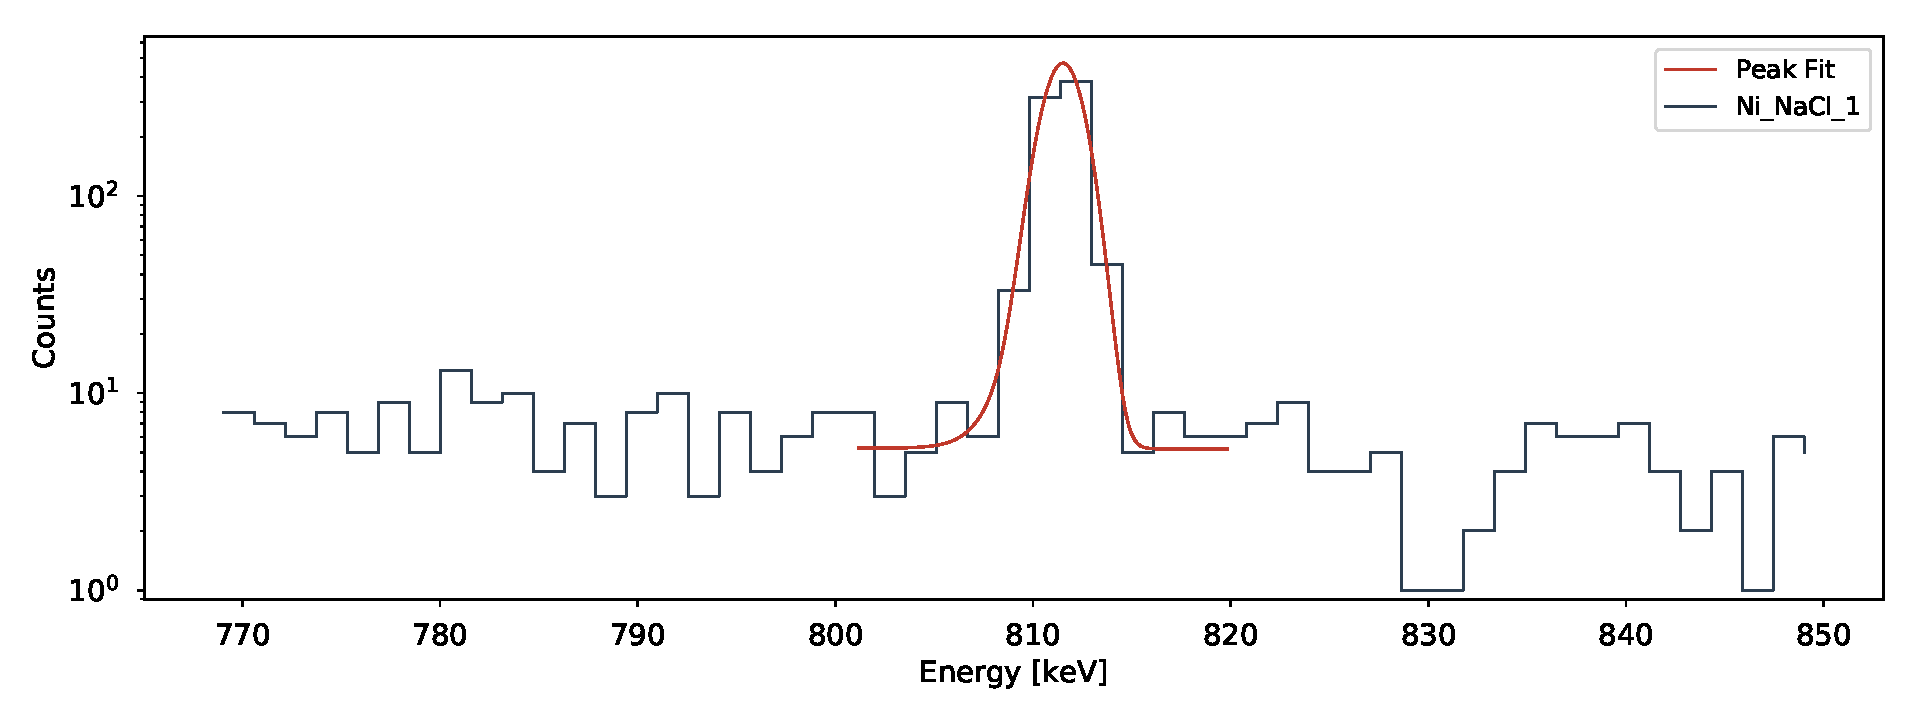
\includegraphics[width=\textwidth]{peak_fits/Ni_NaCl_1.pdf}
\caption{$\gamma$-ray energy spectrum and peak fits in \texttt{\detokenize{Ni_NaCl_1.Spe}}}
\label{fig:Ni_NaCl_1}
\end{figure}

\begin{figure}[htb]
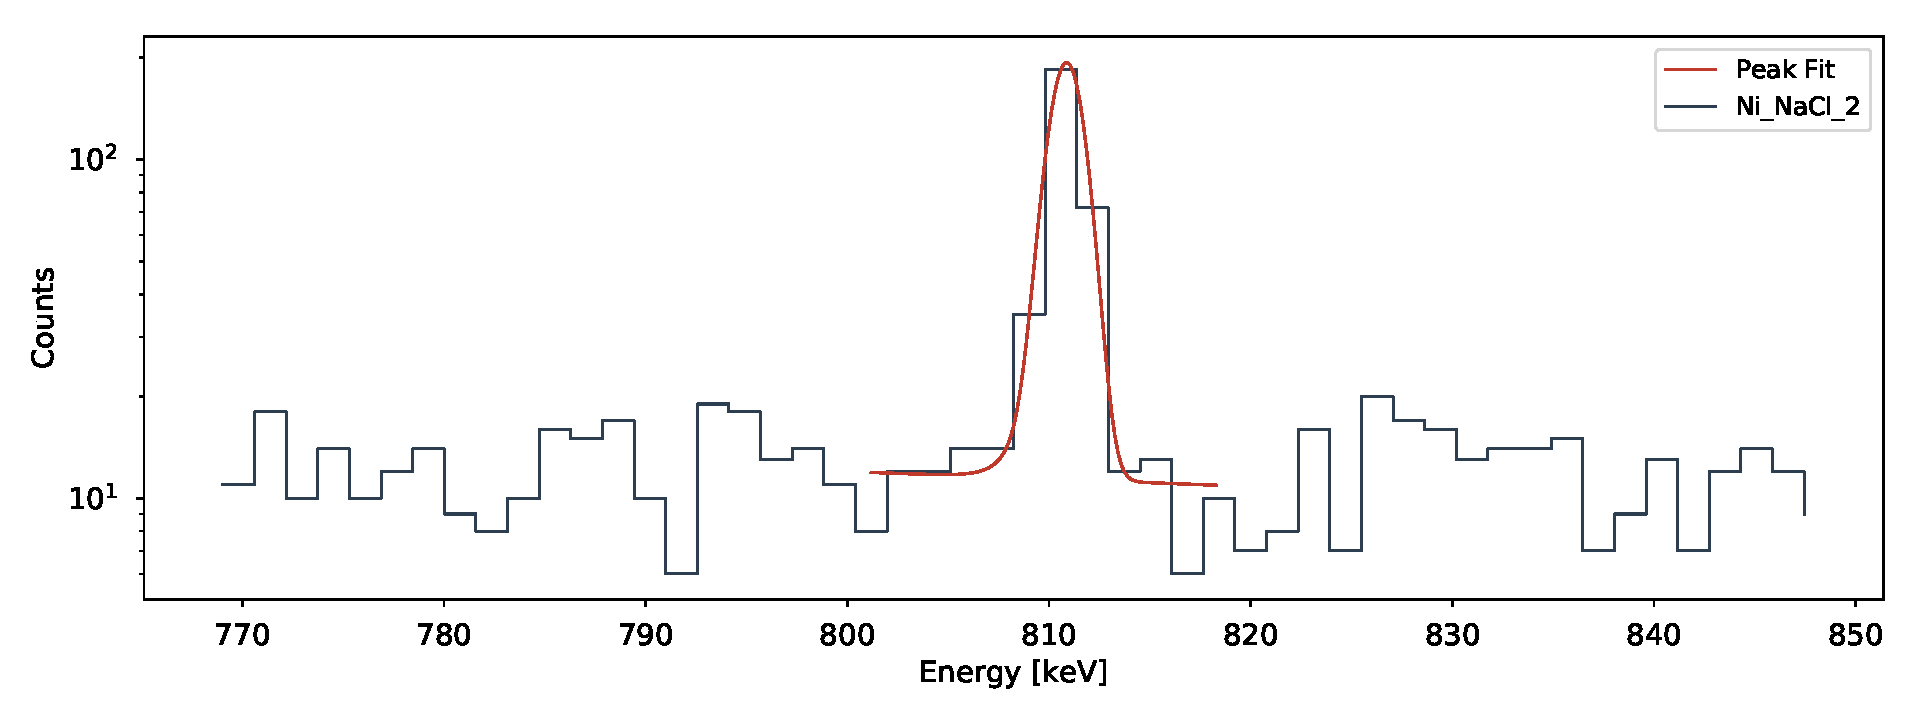
\includegraphics[width=\textwidth]{peak_fits/Ni_NaCl_2.pdf}
\caption{$\gamma$-ray energy spectrum and peak fits in \texttt{\detokenize{Ni_NaCl_2.Spe}}}
\label{fig:Ni_NaCl_2}
\end{figure}

\begin{figure}[htb]
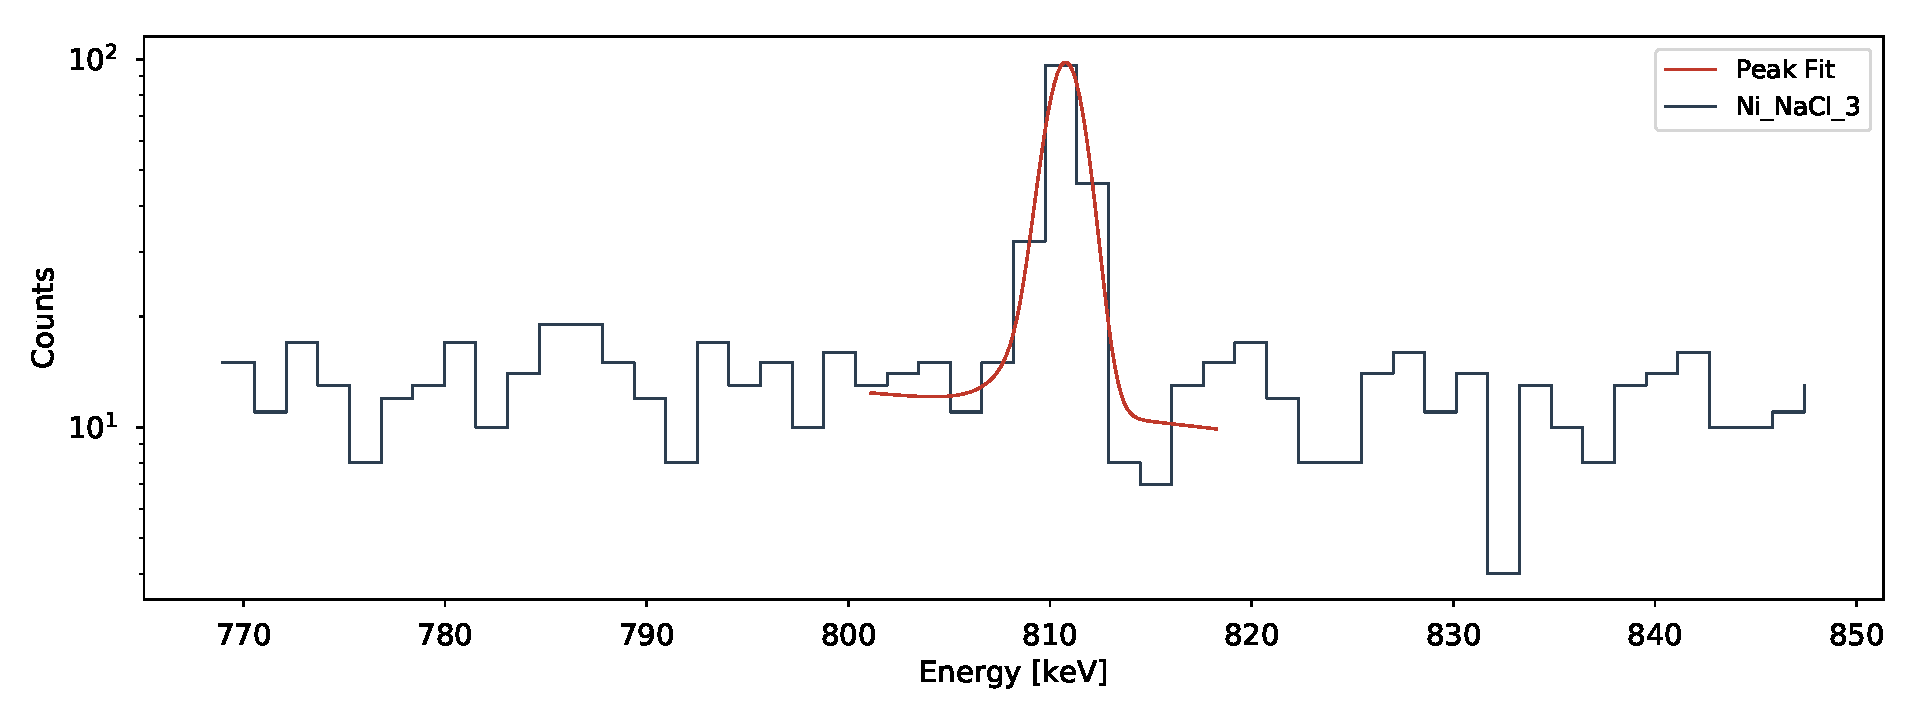
\includegraphics[width=\textwidth]{peak_fits/Ni_NaCl_3.pdf}
\caption{$\gamma$-ray energy spectrum and peak fits in \texttt{\detokenize{Ni_NaCl_3.Spe}}}
\label{fig:Ni_NaCl_3}
\end{figure}

\begin{figure}[htb]
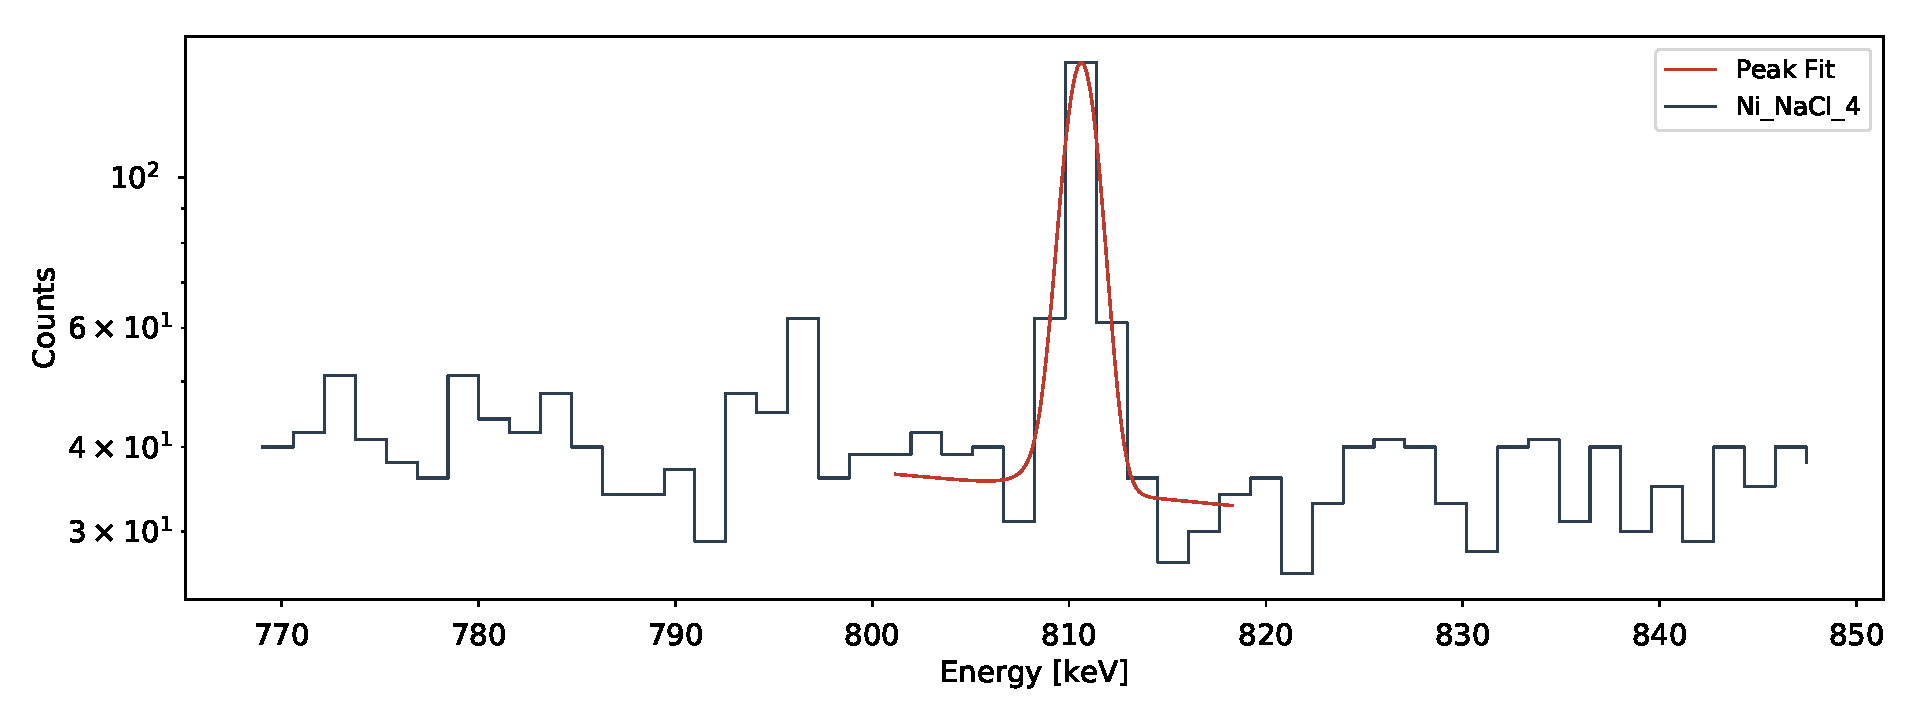
\includegraphics[width=\textwidth]{peak_fits/Ni_NaCl_4.pdf}
\caption{$\gamma$-ray energy spectrum and peak fits in \texttt{\detokenize{Ni_NaCl_4.Spe}}}
\label{fig:Ni_NaCl_4}
\end{figure}

\begin{figure}[htb]
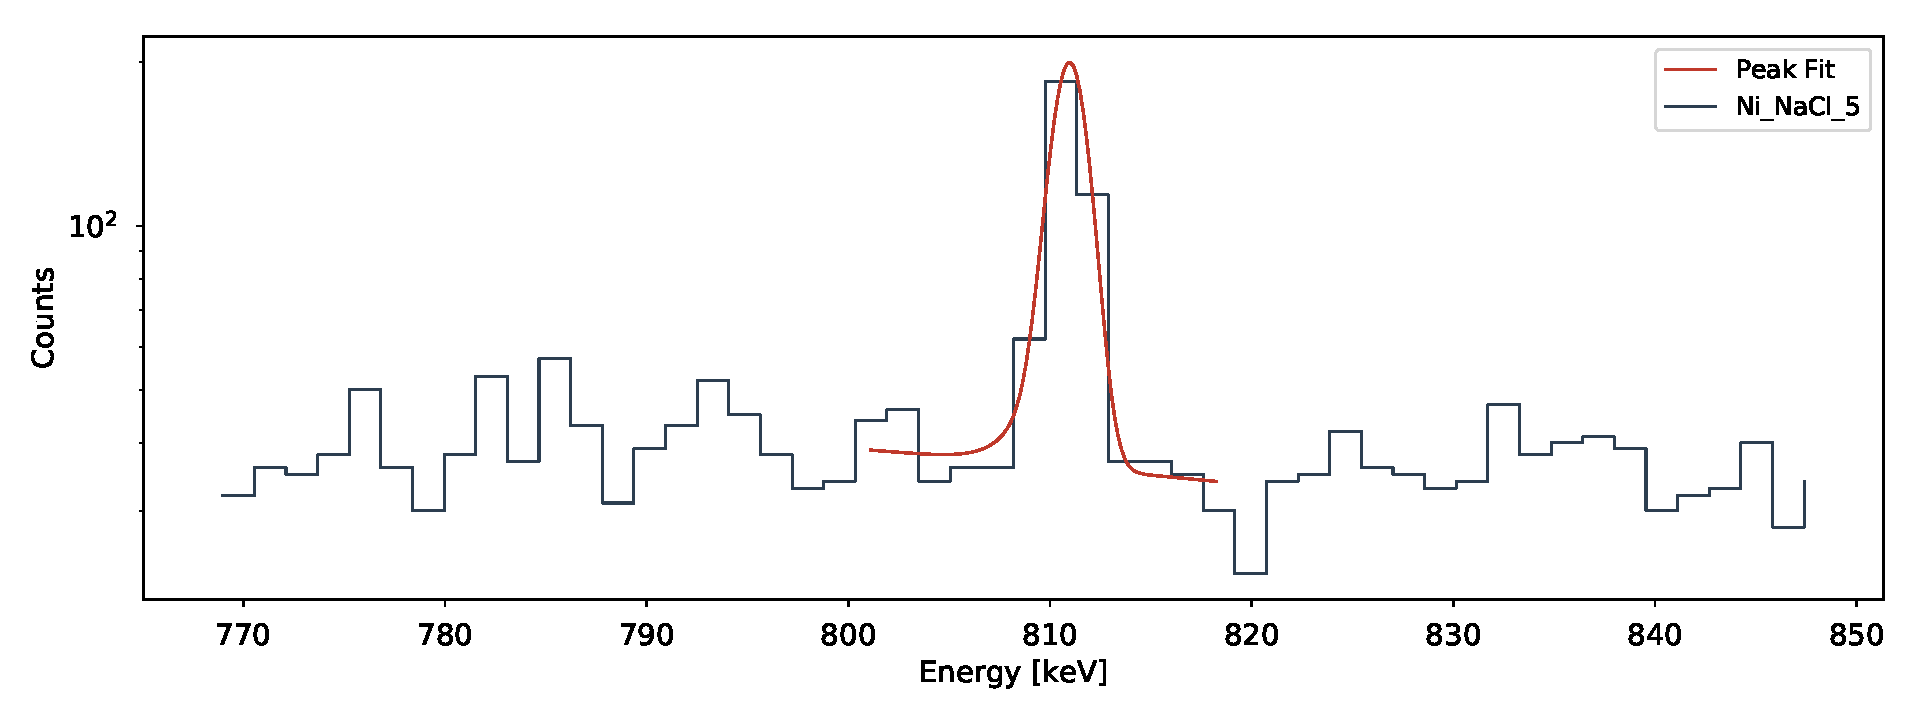
\includegraphics[width=\textwidth]{peak_fits/Ni_NaCl_5.pdf}
\caption{$\gamma$-ray energy spectrum and peak fits in \texttt{\detokenize{Ni_NaCl_5.Spe}}}
\label{fig:Ni_NaCl_5}
\end{figure}



\clearpage
\section{Table of Peaks}
The following table lists the results of the skewed Gaussian peak fits plotted above.  Energy and $I_{\gamma}$ are NNDC values, counts and $\chi^2_{\nu}$ come from the fits. \\

\begin{ruledtabular}
\begin{tabular}{cccccc}
Filename & Isotope & $\gamma$ Energy [keV] & $I_{\gamma}$ & Counts & $\chi^2_{\nu}$ \\
\hline
\texttt{\detokenize{Eu_centered.Spe}} & $^{152}$Eu & 295.9387 & 0.44$\pm$0.44 & 14405$\pm$517 & 3.2 \\
\texttt{\detokenize{Eu_centered.Spe}} & $^{152}$Eu & 329.41 & 0.1213$\pm$0.1213 & 3503$\pm$1260 & 47.4 \\
\texttt{\detokenize{Eu_centered.Spe}} & $^{152}$Eu & 367.7891 & 0.859$\pm$0.859 & 31830$\pm$4042 & 57.8 \\
\texttt{\detokenize{Eu_centered.Spe}} & $^{152}$Eu & 411.1165 & 2.237$\pm$2.237 & 50796$\pm$2468 & 46.5 \\
\texttt{\detokenize{Eu_centered.Spe}} & $^{152}$Eu & 444.01 & 0.298$\pm$0.298 & 11081$\pm$2912 & 13.1 \\
\texttt{\detokenize{Eu_centered.Spe}} & $^{152}$Eu & 443.9606 & 2.827$\pm$2.827 & 58157$\pm$2212 & 13.1 \\
\texttt{\detokenize{Eu_centered.Spe}} & $^{152}$Eu & 488.6792 & 0.414$\pm$0.414 & 7171$\pm$489 & 5.0 \\
\texttt{\detokenize{Eu_centered.Spe}} & $^{152}$Eu & 563.986 & 0.494$\pm$0.494 & 8834$\pm$450 & 1.7 \\
\texttt{\detokenize{Eu_centered.Spe}} & $^{152}$Eu & 566.438 & 0.131$\pm$0.131 & 2550$\pm$397 & 1.7 \\
\texttt{\detokenize{Eu_centered.Spe}} & $^{152}$Eu & 586.2648 & 0.455$\pm$0.455 & 7118$\pm$760 & 7.9 \\
\texttt{\detokenize{Eu_centered.Spe}} & $^{152}$Eu & 656.489 & 0.1441$\pm$0.1441 & 1827$\pm$210 & 0.6 \\
\texttt{\detokenize{Eu_centered.Spe}} & $^{152}$Eu & 674.64 & 0.169$\pm$0.169 & 2212$\pm$407 & 2.3 \\
\texttt{\detokenize{Eu_centered.Spe}} & $^{152}$Eu & 678.623 & 0.473$\pm$0.473 & 5569$\pm$371 & 2.3 \\
\texttt{\detokenize{Eu_centered.Spe}} & $^{152}$Eu & 688.67 & 0.856$\pm$0.856 & 11644$\pm$384 & 2.3 \\
\texttt{\detokenize{Eu_centered.Spe}} & $^{152}$Eu & 719.346 & 0.25$\pm$0.25 & 3402$\pm$1111 & 25.9 \\
\texttt{\detokenize{Eu_centered.Spe}} & $^{152}$Eu & 764.88 & 0.189$\pm$0.189 & 1792$\pm$600 & 7.1 \\
\texttt{\detokenize{Eu_centered.Spe}} & $^{152}$Eu & 778.9045 & 12.93$\pm$12.93 & 152702$\pm$5445 & 199.4 \\
\texttt{\detokenize{Eu_centered.Spe}} & $^{152}$Eu & 810.451 & 0.317$\pm$0.317 & 4117$\pm$271 & 0.9 \\
\texttt{\detokenize{Eu_centered.Spe}} & $^{152}$Eu & 841.574 & 0.168$\pm$0.168 & 1644$\pm$272 & 1.4 \\
\texttt{\detokenize{Eu_centered.Spe}} & $^{152}$Eu & 867.38 & 4.23$\pm$4.23 & 41467$\pm$1424 & 19.0 \\
\texttt{\detokenize{Eu_centered.Spe}} & $^{152}$Eu & 919.337 & 0.419$\pm$0.419 & 3459$\pm$424 & 4.4 \\
\texttt{\detokenize{Eu_centered.Spe}} & $^{152}$Eu & 926.31 & 0.272$\pm$0.272 & 2080$\pm$421 & 4.4 \\
\texttt{\detokenize{Eu_centered.Spe}} & $^{152}$Eu & 963.367 & 0.14$\pm$0.14 & 10535$\pm$19108 & 35.1 \\
\texttt{\detokenize{Eu_centered.Spe}} & $^{152}$Eu & 964.057 & 14.51$\pm$14.51 & 130682$\pm$16941 & 35.1 \\
\texttt{\detokenize{Eu_centered.Spe}} & $^{152}$Eu & 1005.27 & 0.659$\pm$0.659 & 6834$\pm$262 & 1.8 \\
\texttt{\detokenize{Eu_centered.Spe}} & $^{152}$Eu & 1085.837 & 10.11$\pm$10.11 & 94161$\pm$3004 & 90.2 \\
\texttt{\detokenize{Eu_centered.Spe}} & $^{152}$Eu & 1089.737 & 1.734$\pm$1.734 & 12879$\pm$2734 & 90.2 \\
\texttt{\detokenize{Eu_centered.Spe}} & $^{152}$Eu & 1109.18 & 0.189$\pm$0.189 & 9935$\pm$5862 & 20.6 \\
\texttt{\detokenize{Eu_centered.Spe}} & $^{152}$Eu & 1112.076 & 13.67$\pm$13.67 & 108164$\pm$5143 & 20.6 \\
\texttt{\detokenize{Eu_centered.Spe}} & $^{152}$Eu & 1212.948 & 1.415$\pm$1.415 & 9946$\pm$360 & 3.7 \\
\texttt{\detokenize{Eu_centered.Spe}} & $^{152}$Eu & 1249.94 & 0.187$\pm$0.187 & 1451$\pm$150 & 1.5 \\
\texttt{\detokenize{Eu_centered.Spe}} & $^{152}$Eu & 1299.142 & 1.633$\pm$1.633 & 10866$\pm$513 & 16.3 \\
\texttt{\detokenize{Eu_centered.Spe}} & $^{152}$Eu & 1408.013 & 20.87$\pm$20.87 & 136357$\pm$4551 & 229.1 \\
\texttt{\detokenize{Eu_centered.Spe}} & $^{152}$Eu & 1457.643 & 0.497$\pm$0.497 & 3272$\pm$174 & 5.7 \\
\texttt{\detokenize{Eu_centered.Spe}} & $^{152}$Eu & 1528.1 & 0.279$\pm$0.279 & 5827$\pm$253 & 12.0 \\
\texttt{\detokenize{Ni_centered.Spe}} & $^{58}$Co & 810.7593 & 99.45$\pm$9.945 & 17799$\pm$299 & 10.5 \\
\texttt{\detokenize{Ni_centered.Spe}} & $^{58}$Co & 863.951 & 0.686$\pm$0.01 & 110$\pm$25 & 0.8 \\
\end{tabular}
\end{ruledtabular}

\end{document}